\documentclass{ppig}
\usepackage{epsfig}
\usepackage{booktabs}
\usepackage{ucs}
\usepackage{floatrow}
\usepackage[utf8x]{inputenc}
\usepackage[pdfstartview=FitH]{hyperref}
\usepackage{enumitem} 
\setlist[itemize]{noitemsep}


% The titlebox defines how much vertical space is given for
% the authors' list. If you need extra space to show all the
% authors, uncomment the line below and increase the value. Please
% do not make the titlebox smaller than the original size of 5cm.
%\setlength\titlebox{5cm}

\title{Choosers: The design and evaluation of a visual algorithmic music
composition language for non-programmers}

% List the authors like you would in a table.
% The \And command creates another author's column. Use it after the
% details of one author to separate them from the following author horizontally.
% The \AND command creates a new "row" of authors and it should be used
% when the authors don't fit on the same line. You may have to increase
% the titlebox so that the author's don't overlap with the abstract.
\author{Matt Bellingham \\
  Department of Music \\
  University of Wolverhampton \\
%  Faculty of Arts \\
  matt.bellingham@wlv.ac.uk \\
  \And
  Simon Holland \\
  Music Computing Lab \\
%  Centre for Research In Computing \\
  The Open University \\
  s.holland@open.ac.uk \\
  \And
  Paul Mulholland\\
  Knowledge Media Institute \\
%  Centre for Research In Computing \\
  The Open University \\
  p.mulholland@open.ac.uk}

\date{}

\begin{document}
\maketitle
\thispagestyle{empty}

\begin{abstract}
Algorithmic music composition involves specifying music in such a way
that it is non-deterministic on playback, leading to music which has the
potential to be different each time it is played. Current systems for
algorithmic music composition require the user to have considerable
background knowledge of programming and/or music theory. However, much
of the potential user population are self-taught music producers without
the required background in either programming or music. To investigate
how this gap between tools and potential users might be better bridged
we designed Choosers, a prototype algorithmic programming system centred
around a new abstraction (of the same name) designed to allow
non-programmers access to algorithmic music composition methods.
Choosers provides a graphical notation that allows structural elements
of key importance in algorithmic composition (such as sequencing,
choice, multi-choice, weighting, looping and nesting) to be foregrounded
in the notation in a way that is accessible to non-programmers. In order
to test design assumptions a Wizard of Oz study was conducted in which
seven pairs of undergraduate music technology students used Choosers to
carry out a range of rudimentary algorithmic composition tasks. Feedback
was gathered using the Programming Walkthrough method. All users were
familiar with Digital Audio Workstations, and as a result they came with
some relevant understanding, but also with some expectations that were
not appropriate for algorithmic music work. Users were able to
successfully make use of the mechanisms for choice, multi-choice,
looping, and weighting after a brief training period. The stop behaviour
was not as easily understood and required additional input before users
fully grasped it. Some users wanted an easier way to override
algorithmic choices. These findings have been used to further refine the
design of Choosers.
\end{abstract}

\hypertarget{introduction}{%
\section{Introduction}\label{introduction}}

Algorithmic composition typically involves structural elements such as
indeterminism, parallelism, choice, multi-choice, recursion, weighting,
and looping (Jacob, 1996). There are powerful existing tools, such as
Max (Puckette, 1991) and SuperCollider (McCartney, 2002) for
manipulating these and other elements of music. However, while these
systems give great compositional power to musicians who are also skilled
programmers (Wilson, Cottle and Collins, 2011), many musicians who are
not also expert programmers find these tools inaccessible and difficult
to understand and use (Bullock, Beattie and Turner, 2011).

This paper presents an evaluation of a prototype visual programming
language (Bellingham, Holland and Mulholland, 2017) designed to allow
structural elements of the kind involved in algorithmic music
composition to be readily visualised and manipulated, while making
little or no demand on programming ability. This system, called
Choosers, centres around a novel non-standard programming abstraction
(the Chooser) which controls indeterminism, parallelism, choice,
multi-choice, recursion, weighting, and looping.

In this paper we present a programming walkthough evaluation carried out
with six pairs of undergraduate Music Technology students. The purpose
of this evaluation is to:

\begin{itemize}
\item
  Test the ability of self-taught music producers without programming
  skills to use Choosers to carry out a range of rudimentary algorithmic
  composition tasks;
\item
  Identify usability and user experience problems in the current design;
\item
  Identify tensions and trade-offs in the interaction design of the
  system.
\end{itemize}

In the evaluation, pairs of participants were introduced to each element
of the graphical programming language via short tutorial videos.
Participants were given a range of practical tasks to complete on paper
or a whiteboard. The evaluation facilitator played a Wizard of Oz role,
rapidly translating participants' graphical solutions into runnable code
that was fed into a non-graphical prototype version of Choosers so that
participants could hear the musical results of their attempts.

\hypertarget{related-workproblem-setting}{%
\section{Related work/problem
setting}\label{related-workproblem-setting}}

Various music programming languages are capable of algorithmic
composition, although they require significant programming skills
(Bullock, Beattie and Turner, 2011) and are therefore inaccessible to
many users. Bellingham, Holland and Mulholland (2014) used the Cognitive
Dimensions of Notations framework (Green and Petre, 1996) to review the
usability of a representative selection of software capable of
algorithmic music composition. The findings of the review included the
following. First, we found that most existing software requires the user
to have a considerable understanding of constructs in either graphical
(e.g Max, Pure Data) or text-oriented (e.g.~SuperCollider, ChucK,
Csound) programming languages: such knowledge requires a significant
learning overhead. Second, users are often required to have an
understanding of musical notation and/or music production equipment such
as mixing desks and patchbays. Third, several programs imposed working
practices unconducive to compositional processes. Fourth, in some cases
the user was unable to define, and subsequently change, the musical
structure. Finally, complex visual design in graphical programming
languages led to patches with multiple connections, making them
difficult to read and to navigate.

\hypertarget{sec:systemintro}{%
\section{Introduction to the system: Choosers}\label{sec:systemintro}}

The following section provides a brief overview of Choosers, designed to
cover enough detail to allow readers to understand the evaluation. The
participants in the evaluation learned how the system worked by watching
a sequence of short introductory videos and by investigating the system
interactively via Wizard of Oz. For readers convenience the videos can
be found online\footnote{Available at \url{https://goo.gl/PFeAJf}}, and
full details of the system design can be found in Bellingham, Holland
and Mulholland (2017). The system has general musical expressivity, but
for simplicity the present evaluation focuses on the manipulation of
samples for algorithmic composition.

\hypertarget{samples-and-sequences}{%
\subsection{Samples and sequences}\label{samples-and-sequences}}

Samples are shown in boxes, and in the simulated interface can be
auditioned by clicking on them. Samples can be assembled into sequences
using arrows (see fig.~\ref{fig:sequence}). Samples in a sequence play
in the order indicated by the direction of the arrows. Only a single
arrow can enter or exit each element in a sequence. This deliberate
limitation reflects the fact that parallelism and choice are dealt with
elsewhere in the language. Boxes and sequences can be put inside other
boxes, thereby packaging them into a single unit.


\begin{figure}[!h]
	\begin{floatrow}
		\ffigbox{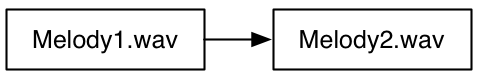
\includegraphics[height=1cm]{./media/image1.png}}
			{\caption{Samples are shown in boxes, and a sequence is assembled via
arrows.}\label{fig:sequence}}
		\ffigbox{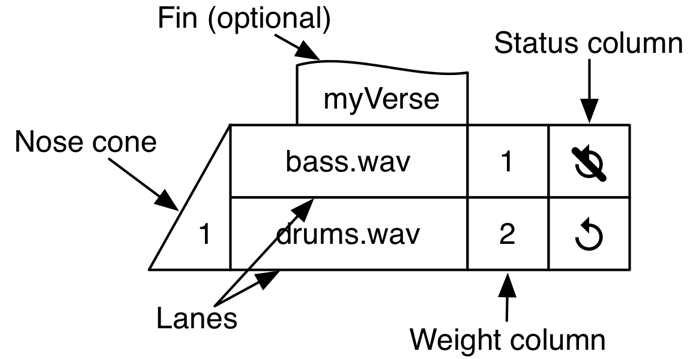
\includegraphics[height=3cm]{./media/image2.png}}
			{\caption{An annotated chooser.}\label{fig:annotated}}
	\end{floatrow}
\end{figure}


\hypertarget{choosers-indeterminism-choice-parallelism-and-multi-select}{%
\section{Choosers: indeterminism, choice, parallelism and
multi-select}\label{choosers-indeterminism-choice-parallelism-and-multi-select}}

Boxes referring to samples or sequences can be snapped together
vertically to create what are known as Choosers (see
fig.~\ref{fig:annotated}).

Fig.~\ref{fig:annotated} shows a Chooser with two lanes, each containing
a sample (drums and bass). The number 1 in the nose cone indicates that
at run time, just one of the lanes will be selected at random (subject
to restrictions described below). On different runs, different choices
may be made. In fig.~\ref{fig:annotated}, by manipulating the number in
the nose cone, any number of lanes from 0 to 2 can be chosen randomly to
play simultaneously. A Chooser can have any number \emph{n} of lanes. By
manipulating the number in the nose cone, any number of lanes from 0 to
\emph{n} can be chosen randomly at run time and played simultaneously.
Each lane has a weight associated with it. Consequently, in
fig.~\ref{fig:annotated}, the drums are twice as likely to be chosen as
the bass. Additionally, a weight of `A' (`always play') can be used to
ensure that the lane is always selected for playback.

\hypertarget{looping}{%
\subsection{Looping}\label{looping}}

Any sample can be set to loop indefinitely when selected on a particular
run, or to play just once by the choice indicated in the status column
(shown in fig.~\ref{fig:annotated}). Indefinite looping of a single
sample may not always be desired, and for this reason we now introduce
Time Choosers (see fig.~\ref{fig:timechooser}).

\begin{figure}[!h]
	\begin{floatrow}
		\ffigbox{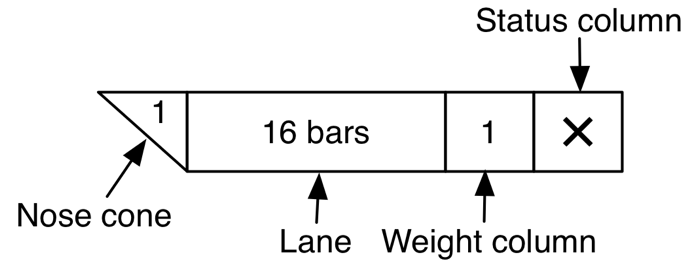
\includegraphics[height=1cm]{./media/image3.png}}
			{\caption{An annotated Time Chooser.}\label{fig:timechooser}}
		\ffigbox{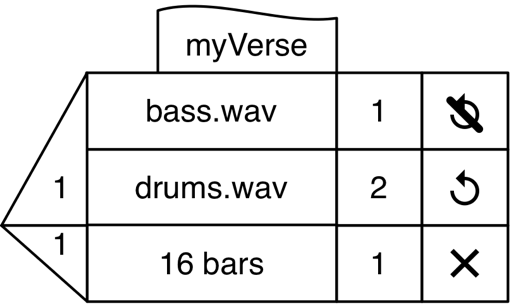
\includegraphics[height=3cm]{./media/image4.png}}
			{\caption{A full chooser.}\label{fig:fullchooser}}
	\end{floatrow}
\end{figure}


\hypertarget{time-choosers-and-full-choosers}{%
\subsection{Time Choosers and Full
Choosers}\label{time-choosers-and-full-choosers}}

If the Time Chooser shown in fig.~\ref{fig:timechooser} is attached onto
the bottom of the Chooser shown in fig.~\ref{fig:annotated}, this
produces the Full Chooser shown in fig.~\ref{fig:fullchooser}.


When the Full Chooser shown in fig.~\ref{fig:fullchooser} is played, if
the looping drums are chosen on a given run, they will not play
indefinitely, but will be cut off after 16 bars by the Time Chooser. If
the Time Chooser duration cleanly divides the sample duration, every
repetition of the sample will run to completion, but if the Time Chooser
duration does not exactly divide by the sample duration (for example, if
the bass.wav sample in fig.~\ref{fig:fullchooser} had a duration of 3
bars), the Time Chooser would cut playback mid-sample.

If, in a run of fig.~\ref{fig:fullchooser}, the non-looping bass were to
be chosen, the bass sample would play once, and if this sample were less
than 16 bars long, there would be silence until the end of the sixteen
bars were reached.

\hypertarget{hard-vs.soft-stop-of-loops}{%
\subsection{Hard vs.~soft stop of
loops}\label{hard-vs.soft-stop-of-loops}}

If the status column in the time chooser is set to \(>\) (indicating a
soft stop) rather than \(\times\) (indicating a hard stop) then, when
the time chooser ends, the sample will continue to play until the end of
its current loop.

\hypertarget{terminology-soundable-choosers-time-choosers-and-full-choosers}{%
\subsection{Terminology: Soundable Choosers, Time Choosers and Full
Choosers}\label{terminology-soundable-choosers-time-choosers-and-full-choosers}}

Now that Time Choosers and Full Choosers have been introduced, in order
to avoid ambiguity, we will refer to Choosers with no attached Time
Choosers, such as those shown in fig.~\ref{fig:annotated}, as Soundable
Choosers.

\hypertarget{time-choosers-on-their-own}{%
\subsection{Time Choosers on their
own}\label{time-choosers-on-their-own}}

A Time Chooser can be used alone as part of a sequence -- however, when
used in this way it will simply result in a rest of the specified
duration.

\hypertarget{time-choosers-with-multiple-lanes}{%
\subsection{Time Choosers with multiple
lanes}\label{time-choosers-with-multiple-lanes}}

More generally, the purpose of a Time Chooser within a Full Chooser is
to moderate in a non-deterministic manner how long the Soundable Chooser
and its individual lanes play. Possible interactions between the
settings of soundable and Time Choosers can make the results more varied
than might be imagined.

A Time Chooser's nose cone can be set to either one or zero. If set to
one, one time lane will be chosen at run time. If it is set to zero no
time lanes will be selected and the Soundable Chooser will run as though
there is no Time Chooser. This allows for quick low viscosity
arrangement changes, with the possibility of infinite playback if the
Soundable Chooser lanes are set to loop. If the Soundable Chooser is not
set to loop, the sample(s) will play and the Chooser will be released
when they have finished playing, regardless of length.

\hypertarget{method}{%
\section{Method}\label{method}}

\hypertarget{participants}{%
\subsection{Participants}\label{participants}}

Seven pairs of undergraduate Music Technology students took part in user
tests utilising a Wizard of Oz prototyping methodology. These users were
targeted as they are typically neither programmers nor traditional
musicians. While they may be conversant with some elements of music
theory, the predominant background is self-taught music producers with
experience of making music electronically using music sequencers/DAWs.
The users were introduced to each element of the graphical programming
language via short tutorial videos\footnote{Available at
  \url{https://goo.gl/PFeAJf}}. Users were given a range of practical
tasks to complete on paper (see fig.~\ref{fig:paper}) or on a
whiteboard, and their outputs were played by the facilitator using a set
of SuperCollider (McCartney, 2002) classes written to implement the
musical abstractions behind the system. The user tests were videoed and
transcribed to assist in the analysis presented here.

All participants were asked to complete a short questionnaire before
taking part in the user tests. Of the fourteen participants all were
musicians, and ten had some formal training. Six participants did not
read any music notation: of those that did, most could read common music
notation as well as chord notation. All participants were familiar with
DAWs, with Logic Pro (Apple Inc., 2013) mentioned by all fourteen users.
Other DAWs mentioned included Pro Tools (6 mentions), Cubase (2
mentions), FL Studio (5 mentions), Reason (1 mention), and Ableton Live
(1 mention). Pure Data (Puckette, 1997) a visual audio programming
language, was mentioned by two participants. Twelve participants had
experience using hardware for music performance HCI tasks (such as drum
pads or control surfaces). The participants were not habitual
performers; seven of the fourteen participants do not perform with or
for others. Of those that do, three perform in church, and four
occasionally play with friends in private. Five of the fourteen
participants felt they had some experience in computer programming. Of
these, two considered writing for the web (HTML and CSS) to be
programming. Given that HTML/CSS development is focussed on markup and
layout we can see that more than two thirds of participants do not have
experience of writing algorithms in a programming language. One
participant listed the use of Pure Data and SuperCollider. Eight of the
fourteen participants did not know what algorithmic music was at the
start of the user tests. Four participants felt that they knew what
algorithmic music was, but had not created any.

\begin{figure}[!h]
	\begin{floatrow}
		\ffigbox{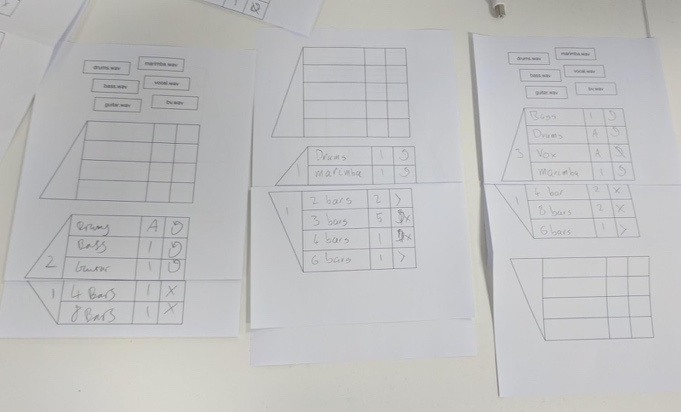
\includegraphics[height=1cm]{./media/image5.jpeg}}
			{\caption{Participant Chooser work using paper.}\label{fig:paper}}
		\ffigbox{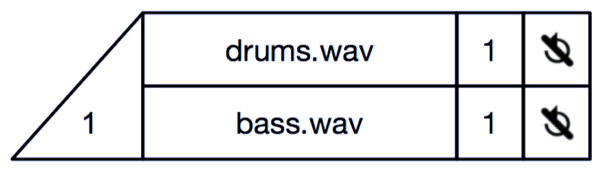
\includegraphics[height=3cm]{./media/image6.png}}
			{\caption{Scenario one.}\label{fig:scenario1}}
	\end{floatrow}
\end{figure}


\hypertarget{walkthrough-protocol}{%
\subsection{Walkthrough protocol}\label{walkthrough-protocol}}

Participants were asked to take part in eight scenarios, as reproduced
below. The users were free to discuss the work and to ask for
clarification with the administrator of the test. Users were asked to
act as active participants in the research, and to help in categorising
any issues that were raised The categorisations that users were asked to
use --taken from the programming walkthough method (Bell, Rieman and
Lewis, 1991; Bell et al., 1992) -- were questions (e.g.~why does the
loop do that?), problems (e.g.~I don't understand what these lanes are
for), suggestions (e.g.~maybe the cone should be a different shape), and
other observations (e.g.~I like the fins). In addition, participants
were asked if they could think of any other ways in which each scenario
could be completed. This prompted a discussion on alternative routes in
order to test understanding and to capture user expectations.

\hypertarget{walkthrough-scenarios}{%
\subsection{Walkthrough scenarios}\label{walkthrough-scenarios}}

We now present the eight scenarios issued as part of the user tests. The
videos, images, and verbal instructions issued to participants are shown
in boxes. This section includes a brief overview of the results from
each scenario. A more detailed reflection on the design issues is in
sec.~\ref{sec:reflection}.

\hypertarget{scenario-1---understanding-the-soundable-chooser}{%
\subsubsection{Scenario 1 - understanding the Soundable
Chooser}\label{scenario-1---understanding-the-soundable-chooser}}

Participants were shown a short video\footnote{Available at
  \url{https://youtu.be/gFbWz-F-WmE}} which introduced lanes, nose cone,
weighting inc. always play, and loop/non-loop functionality.

Here is a Soundable Chooser with two samples.

\begin{itemize}
\item
  If this Chooser is played by itself, how many samples will play?
\item
  How do you know?
\item
  How likely is it that the drums.wav sample will play? How could you
  make it more likely to play?
\item
  How could you make the Chooser play both samples?
\item
  How would you make it play no samples?
\end{itemize}

This scenario prompted a number of clarifying questions from
participants, all of which could be answered simply by playing the video
again. All participants were able to complete this scenario without
error.

\hypertarget{scenario-2---creating-a-soundable-chooser}{%
\subsubsection{Scenario 2 - creating a Soundable
Chooser}\label{scenario-2---creating-a-soundable-chooser}}

Make a Soundable Chooser which has three lanes -- those lanes should
contain looping drums, bass and guitar samples. Make it so that two play
at once -- the drums always play, and either bass or guitar will be
selected with equal probability.

\begin{figure}[!h]
	\begin{floatrow}
		\ffigbox{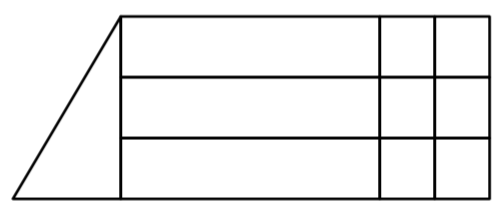
\includegraphics[height=1cm]{./media/image7.png}}
			{\caption{Paper template given to participants for scenario 2.}\label{fig:scenario2}}
		\ffigbox{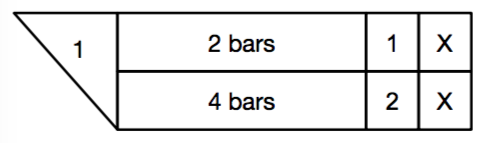
\includegraphics[height=3cm]{./media/image8.png}}
			{\caption{Scenario 3.}\label{fig:scenario3}}
	\end{floatrow}
\end{figure}


\begin{itemize}
\item
  Make it so the guitar doesn't play
\end{itemize}

The Soundable Chooser design was understood quickly by most
participants. The layout of the Chooser -- vertically stacked lanes --
prompted some interesting assumptions from participants in two groups.
The participants appeared to apply existing knowledge of
horizontally-scrolling DAWs, such as Pro Tools or Logic Pro, in which
vertically stacked lanes play concurrently. However, in the Chooser
design, such lanes contain material which may or may not be selected for
playback and concurrency cannot be assumed without also considering the
number in the nose cone, the lane weight, and the ``always'' feature
described below. This assumption, made twice in the user tests, was
corrected at the start of the test and users did not encounter any
further problems.

The use of `A' (`always play') in the weight column of Soundable Chooser
lanes was understood quickly by all participants. Users were asked to
prevent the guitar from being available for selection, and all groups
chose to change the guitar's weight to zero. This answer was correct,
but was not the only way to achieve the desired result. One participant
correctly suggested that the bass could also be set to A, meaning that
the guitar would not be selected given the restriction imposed by the
number in the nose cone.

\hypertarget{sec:scenariothree}{%
\subsubsection{Scenario 3 - understanding the Time
Chooser}\label{sec:scenariothree}}

Participants were shown a short video\footnote{Available at
  \url{https://youtu.be/p03--FbA_r0}} which introduced Time Choosers,
multiple lanes, and nose cone restrictions.

Here is a Time Chooser with two lanes.

\begin{itemize}
\item
  Describe what will happen when this Chooser is run by itself.
\item
  The nosecone is currently set to 1. What else could it be set to? What
  would happen if it is changed?
\item
  How could you make a duration of 2 bars most likely to be selected?
\end{itemize}

Two groups found multiple vertically aligned lanes confusing, as in the
previous scenario. One participant assumed that both durations would
play together, presumably due to the behaviour learned through the use
of DAWs. Another user thought that the first duration would play,
followed by the second duration. In both cases the participants were
shown the relevant section of the tutorial video again, and they then
fully understood the Time Chooser mechanism.

\hypertarget{scenario-4---creating-a-single-lane-time-chooser}{%
\subsubsection{Scenario 4 - creating a single-lane Time
Chooser}\label{scenario-4---creating-a-single-lane-time-chooser}}

Keeping the Soundable Chooser you made for scenario 2, create a
single-lane Time Chooser.

\begin{figure}[!h]
	\begin{floatrow}
		\ffigbox{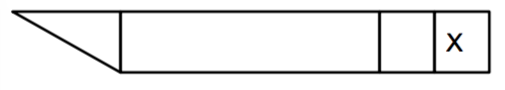
\includegraphics[height=1cm]{./media/image9.png}}
			{\caption{Paper template used for scenario 4.}\label{fig:scenario4}}
		\ffigbox{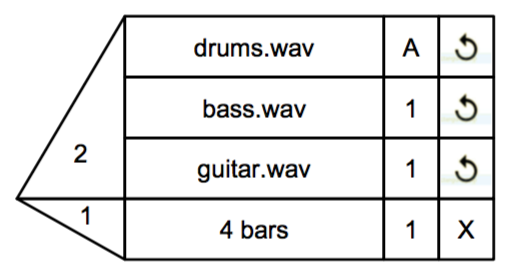
\includegraphics[height=3cm]{./media/image10.png}}
			{\caption{The result of the final task in scenario 4.}\label{fig:scenario4end}}
	\end{floatrow}
\end{figure}


\begin{itemize}
\item
  Make a four bar rest.
\item
  Now you have made the rest, find two ways to quickly skip it. What do
  you think the nose cone value could be? What would happen if you gave
  the nose cone that value?
\item
  What impact would there be if you changed the weight of the lane?
\end{itemize}

Participants were shown a video\footnote{Available at
  \url{https://youtu.be/8AWcolOMMwY}} which introduced Full Choosers,
duration control via the Time Chooser, and the hard and soft stop
mechanism.

\begin{itemize}
\item
  Next, take the Time Chooser and snap it onto the Soundable Chooser
  created in scenario 2. What is the impact of this?
\end{itemize}


The user tests were designed to introduce a Time Chooser as playing
silence for a given duration or, from an alternative viewpoint,
introducing a musical rest. We subsequently moved on to introduce the
Time Chooser's fundamental role, which is to provide a mechanism for
constraining the duration of a Soundable Chooser. We found that
introducing Time Choosers in this way created some confusion among
users, and future user testing will reverse the order in which the two
functions are introduced. Four of the six groups found that the rest
functionality of the Time Chooser was not obvious, although all
participants were able to use it effectively after discussion. When the
user test moved on to the use of a Time Chooser to control a Full
Chooser's duration one participant interpreted it as a rest -- they
continued to use the logical framework of rests rather than
re-contextualise the functionality in the Full Chooser. Tellingly, a
significant number of participants guessed that Time Choosers would be
used to control the duration of Soundable Choosers before the
functionality was introduced. We consider this in more detail in
sec.~\ref{sec:programming}.

Conceptually, hard and soft stops were understood immediately by half of
the participants. These users were able to make musical use of both stop
types. Those who did not initially understand the difference were almost
all able to clarify the stop behaviour via a short discussion. One
participant was surprised by hearing the effects of a soft stop in his
group's final scenario work (`why isn't it stopping?'), prompting
another conversation. The stop functionality is further explored in
sec.~\ref{sec:musical}.

Two groups felt that, while the icon for a hard stop was understandable,
the icon for a soft stop did not make its function clear. When the
intention behind the icon choice was explained (\(\times\) as a hard
stop as it mirrors a `stop' road sign, \(>\) as a soft stop as it looks
like an arrow to allow the material to continue) some participants felt
that it was more understandable. One participant remained unsatisfied
with the soft stop icon, although they could not offer an alternative.

Just as the icon choice had an effect on learnability, the language used
for the stops also seems to have been significant. For those
participants who did not immediately understand the stop functionality
we explained hard stops as `rude' and soft stops as `polite'. These were
the original names used in early development, and they were useful in
allowing the participants to contextualise the stop behaviour. It is not
clear from this process whether one name is more descriptive or
learnable than the other, as not all participants were introduced to
these terms and those who were, encountered them as a secondary
adjective term to support the `hard' and `soft' terminology.

\hypertarget{sec:scenariofive}{%
\subsubsection{Scenario 5 - understanding a Full
Chooser}\label{sec:scenariofive}}

Look at this Chooser and say what will happen when the Chooser is
played. The drums and bass samples are four bars long. The marimba
sample is two bars long.


\begin{figure}[!h]
	\begin{floatrow}
		\ffigbox{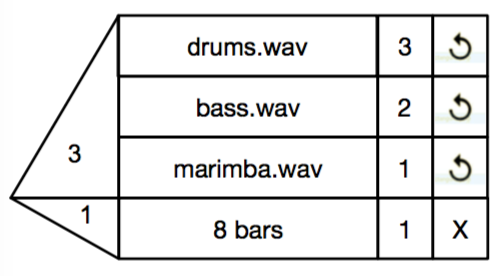
\includegraphics[height=1cm]{./media/image11.png}}
			{\caption{Scenario 5.}\label{fig:scenario5}}
		\ffigbox{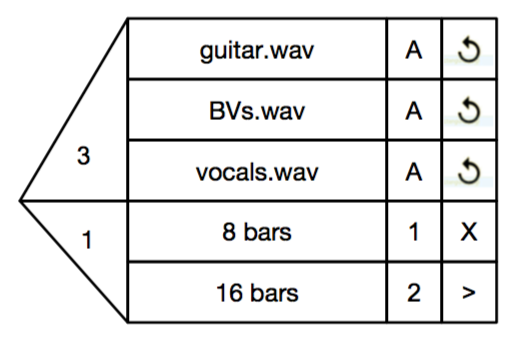
\includegraphics[height=3cm]{./media/image12.png}}
			{\caption{Scenario 6.}\label{fig:scenario6}}
	\end{floatrow}
\end{figure}

\begin{itemize}
\item
  How many samples will play? Will they loop or play once? What effect
  would changing the loop setting on the drums have?
\item
  How long will the Chooser play for? What happens when the duration
  elapses?
\item
  What would happen if the Time Chooser was set to a soft stop?
\item
  What would happen if the Time Chooser nose cone stayed at 1 and the
  Soundable Chooser nose cone was changed to 2? To 1? To zero?
\item
  How could you make it infinite playback? How could it be made into a
  rest? Skipped entirely?
\end{itemize}

When asked to produce a Full Chooser which allows for infinite playback,
the users were expected to set the Time Chooser's nose cone to 0 in
order to prevent it from controlling the Soundable Chooser's duration.
One user wanted to be able to set the time lane's duration to
\(\infty\). While not one of our options, this would potentially be a
valid input. Two participants wanted to use the `A' (always play)
mechanism to set infinite playback -- their logic was that they wanted
to override the set duration. Another user wanted to be able to loop the
Time Chooser to create infinite playback.

One user wanted Soundable Choosers to segment to show the number of
loops in a given duration. For example, if a duration of 8 bars was
selected, and the upper soundable lane contained a 2-bar sample and the
lower lane contained a 4-bar sample, the upper lane would show 4
segments and the lower lane would show 2 segments.

One group were interested in visual feedback from the Choosers. They
wanted to have a progress bar, which presents some interesting
trade-offs and challenges to the system. This is explored in
sec.~\ref{sec:musical} and sec.~\ref{sec:programming}.

\hypertarget{sec:scenariosix}{%
\subsubsection{Scenario 6 - understanding a Full Chooser with multiple
lane times}\label{sec:scenariosix}}

Here is a Chooser containing a Time Chooser with multiple lanes.

\begin{itemize}
\item
  What do you expect to happen in the Soundable Chooser?
\item
  What will happen in the Time Chooser? Which lane is more likely to be
  selected? What are the consequences of the selection of the uppermost
  Time Chooser lane? What will be different if the lower Time Chooser
  lane is selected?
\item
  What other values are possible for the nose cone of the Soundable
  Chooser?
\item
  What other values are possible for the nose cone of the Time Chooser?
\end{itemize}

This scenario, which introduced multiple Time Chooser lanes, was
incorrectly explained by two user groups (see
sec.~\ref{sec:scenariothree}) who did not understand the lane selection
mechanism. This error may be linked to the application of an
understanding of horizontally-scrolling DAWs (see
sec.~\ref{sec:shared}). The use of numbers for multiple parameters may
also have made the functionality unclear (see
sec.~\ref{sec:arithmetic}).

This scenario asked users to consider the possible nose cone values
given three Soundable Chooser lanes with a weight of `A' (always play).
The correct answer (either three to play all lanes, or zero to skip the
Soundable Chooser) was quickly identified by most participants. Two
groups questioned the semantic logic of allowing the `always play'
directive to be overridden and, if it can be overridden, why this can be
only performed in one context. This was an interesting example of users
applying their knowledge from within the system and is considered in
more detail in sec.~\ref{sec:shared}. The issue is indeed problematic
and led to the infinity option discussed in more detail in
sec.~\ref{sec:solutions}. The infinity option proposed in
sec.~\ref{sec:solutions} does not require the nose cone to be changed or
constrained, while allowing similar semantic meaning.

\hypertarget{scenario-7---creating-a-full-chooser}{%
\subsubsection{Scenario 7 - creating a Full
Chooser}\label{scenario-7---creating-a-full-chooser}}

Using the templates (provided on paper), create a Full Chooser which:

\begin{itemize}
\item
  Has four soundable lanes, three of which will play at any given time.
  Drums and bass, which always play, and are set to loop: guitar and
  vocals, where the guitar is twice as likely as vocals to be selected
  for playback. Neither should loop.
\item
  Has three possible durations, of which one will be selected -- 2 bars
  with a hard stop, 4 bars with a soft stop, and 5 bars with a hard
  stop. Make the 2 bar duration twice as likely to be selected as the 4
  and 5 bar durations.
\end{itemize}

This task was performed quickly and accurately by all groups. The users
in two groups requested preset Choosers to enable them to build a viable
piece of music quickly. Presets could also provide tutorial support by
providing a framework around which users could experiment.

\hypertarget{scenario-8-playground}{%
\subsubsection{Scenario 8 -- playground}\label{scenario-8-playground}}

Users were shown the final video\footnote{Available at
  \url{https://youtu.be/bBnngW-W_HU}} which introduced the sequence
mechanism.

Using the templates and samples available, make a piece of music which
uses a sequence of three Choosers. The music will be recorded and shared
online. The piece should be musically satisfying even if it is run only
once. If it is run more than once it should be different in some way.

The participants were able to create some interesting musical material,
and all enjoyed hearing the results of their work. This was the first
time that any of them had created algorithmic music. Three participants
felt that the user interface used numbers for too many parameters. Upon
questioning, their concern was that there was insufficient
differentiation between quite different user interface elements, making
the interface both difficult to learn and confusing in operation.
Numbers are used in the nose cone, the time lanes (e.g. `8 bars'), and
the weight column. We consider this in sec.~\ref{sec:arithmetic}.

One suggestion was to change the Time Chooser nose cone to an on/off
icon given that the only legal options were zero and one. It is
interesting to note that some users were able to identify that a Boolean
value is required here, and we consider the implications of this in
sec.~\ref{sec:solutions}.

Most users used this final task to test their understanding of the
system, rather than creating a cohesive piece of music. Of the seven
groups, one decided to create a piece which developed thematically. To
do this they wanted to reuse a Chooser, making minor changes to it. We
discussed copying the original Chooser, and this process met their
requirements.

One group was interested in reusing some elements of the composition
created in the final scenario, and so we discussed the nesting
functionality which was left out of this round of user testing (see
Bellingham, Holland and Mulholland (2017) for an explanation of nesting
in Choosers). They understood the concept and it entirely met their
requirements.

\hypertarget{final-questions}{%
\subsubsection{Final questions}\label{final-questions}}

At the end of the user test, participants were asked the following three
questions:

\begin{itemize}
\item
  Can you see anything this would be useful for?
\item
  Can you see any ways in which this is similar to other tools you have
  used?
\item
  Is there anything that is made easier by this system? Anything which
  was not possible made possible/hard and made easier?
\end{itemize}

Three groups commented on the `boring' design. The layout of Choosers
was not seen as problematic, but some users wished for a more stylish
and polished presentation. Two groups requested colours to enhance
usability: within one group, one user wanted automatic colour selection
(denoting lane type) and the other user felt that user-controlled colour
selection would better support sorting and arrangement tasks. Multiple
users were interested to know if lanes could be rearranged to visually
organise lanes into instrument groups. One user suggested that lane
arrangement could be an alternative to the weight column --- moving a
lane higher would result in a higher probability of playback. This is
similar to one mechanism which was considered and rejected before the
user tests: it was replaced by the weight column as the column allows
for multiple identical lane weights, quick auditioning, and
user-controlled lane ordering to assist with musical arrangement. One
user requested instrument icons for soundable lanes, partly in response
to being unaware of the marimba (one of the samples used in the user
test).

\hypertarget{sec:reflection}{%
\section{Reflection on design issues}\label{sec:reflection}}

The findings from the user tests outlined above have various
implications for the design of Choosers.

\hypertarget{sec:musical}{%
\subsection{Musical issues}\label{sec:musical}}

Repeating phrases, and the musical interaction between phrases, are
crucially important in a music system. These have therefore been brought
to the surface via the loop and hard/soft stop behaviours. We found that
the stop behaviour was confusing to four of the seven pairs of users,
and the documentation will be enhanced to better explain the system. The
hard and soft stop system can be thought of in a number of ways. For
musicians, one useful way is to consider soft stops as suitable for
melodies, and hard stops for accompaniment. Melodies are therefore
allowed to finish, whereas accompanying elements are stopped when the
duration of the Chooser elapses.

Three of the fourteen users were keen to have a visual indication of
current position with respect to duration, such as a progress bar. While
this seems a reasonable request, it is complicated by the
non-deterministic nature of the system.

A significant number of participants found the use of Time Choosers for
both rests and Chooser duration to be confusing. This was largely due to
rests being introduced before the Time Chooser's primary function, which
is to control the duration of a Chooser.

None of the participants had experience in algorithmic composition, so
these sessions essentially introduced algorithmic compositional tools
while testing the interface. This led some participants to presume that
the concepts themselves were novel. Some time was spent discussing the
desirability of algorithmic processes rather than this specific
implementation. Two participants assumed that the process would lead to
a linear audio file, which indeed it can, but many use cases would
require the music to remain nonlinear. Future evaluations could explore
the nature of the resistance to nonlinear playback, including how it is
related to expectations set by commercial music creation software and
linear playback. We are also interested in the use of Choosers in genres
which routinely incorporate extemporaneous changes and improvisation,
such as folk and jazz.

One group specifically wanted a mechanism to allow them to easily reuse
material for thematic development. The design of Choosers allows for
this via nesting, although it was not included in the user tests for
simplicity. The users were shown nesting in response to their questions
and found it to meet the need they had expressed.

Choosers can be used in the creation of a range of music. However, given
the unusual combination of usability and affordances, Choosers are
particularly suited to music in which users would benefit from easy
access to non-linear playback. Some classic Minimalism techniques
(Potter, 2002), such as phasing (Scherzinger, 2005), are easily
achievable using Choosers. Game music is often non-linear, created using
layers of musical material which are triggered by in-game events
(Collins, 2008). Such material can be created using Choosers, and we
have a mechanism which would allow for external input via OSC or an
alternative protocol; this would allow a game engine to trigger changes
in the music. Choosers also allow musicians and music producers to
create nonlinear versions of existing recordings by loading alternate
takes into Choosers. The playback could range from very close to the
original (e.g.~algorithmically switching between vocal takes of the same
melody) to playing significantly different material (e.g.~branching to
play different sections), depending on the decisions made by the
creators.

\hypertarget{sec:programming}{%
\subsection{Programming-related issues}\label{sec:programming}}

As shown in sec.~\ref{sec:systemintro}, the Soundable Chooser nose cone
slopes down and the Time Chooser nose cone slopes up -- this allows them
to be joined together and communicates the required upper/lower order to
the user. Interestingly, some users guessed the combination of Soundable
and Time Choosers, suggesting that the nose cone shapes of the two
Chooser types were effective in communicating their combinatorial usage.

The Chooser system is designed to allow for consistent logic to be
applied across Soundable and Time Choosers where possible. Participants
in the user tests successfully reused elements of the Soundable Chooser
system when manipulating duration, but there were some cases where such
reuse or re-contextualisation was not possible. Interestingly, the
actions of the users in these cases would have made sense neither from a
musical nor programming perspective, but the rationale behind these
requests is instructive as it shows how users understand the tools in
the system. For example, in scenario five (sec.~\ref{sec:scenariofive})
two participants wanted to use the `A' (always play) mechanism to set
infinite playback -- they wanted to override the set duration and had
understood `A' to be a global override control. In a similar example,
one user wanted to be able to loop a Time Chooser. If the system were to
be changed to allow for a set number of repeats, rather than an infinite
loop, such a move may be desirable.

Users will also require access to metadata -- for example, to check the
length of a sample loaded into a soundable lane in a Chooser. Such
metadata could be shown via a tooltip, accessed by hovering the mouse
over a lane.

\hypertarget{sec:shared}{%
\subsection{Shared and existing knowledge}\label{sec:shared}}

One design motivation is to enable people to understand the system very
quickly. The Chooser design tacitly draws on a number of systems of
existing knowledge.

Some users wanted to be able to leverage their existing understanding of
DAW software and found it frustrating that they needed to learn new
paradigms for duration, synchronicity, and so on. This is an example of
technological framing (Orlikowski and Gash, 1994). The knowledge gained
by using other music software can be useful, but it can also prove
problematic if the design of the software being learned is sufficiently
differentiated. As a result, there is much to be gained by following
standard design conventions where possible, as this maximises the user's
ability to reuse existing knowledge. One interesting example was seen in
scenario 6 (sec.~\ref{sec:scenariosix}), in which one pair of users
learned the rules of Choosers and then wanted to use the same rules
elsewhere.

Technological framing, and the expectations set by the use of commercial
DAWs, may be an influence on user requests for a progress bar and the
conversations on the desirability of nonlinear vs.~linear playback that
took place during the user tests (as considered in
sec.~\ref{sec:musical}).

\hypertarget{sec:metaphor}{%
\subsection{Metaphor}\label{sec:metaphor}}

Interface metaphors are very common and can be useful in communicating
the roles of the software and setting realistic expectations when users
are familiar with the original interface. However, such metaphors can
become problematic if users are not familiar with the original
interface.

Related to technological framing is the assumption, ubiquitous in
Digital Audio Workstations, that signal flow and processing will be
applied using a mixing desk metaphor. Such virtual desks often make use
of skeuomorphism (such as the fader caps and rotary potentiometers in
Pro Tools), although some other designs have made graphical changes
while retaining the overall layout. As an example, Ardour's use of a
textured `strip' instead of a fader is still skeuomorphic as it makes
use of a ribbon controller metaphor but, in an attempt to improve mouse
control by increasing the size of the target, it does not follow the
traditional desk layout.

Given that DAWs are now capable of performing all mixdown tasks, and the
financial cost of consoles and outboard effects processors can be
prohibitive, many users learn in a virtual studio environment rather
than on hardware. Many DAWs were designed to mimic hardware in order to
leverage existing knowledge and ease the transition from hardware to
software. However, now most people are introduced to music production
via software, and many do not use hardware, there is an opportunity to
revisit some design assumptions.

Some users felt that the user interface was `boring', lacking the use of
colour, metaphor, and skeuomorphic design common in DAWs. This may be
another example of technological framing (Orlikowski and Gash, 1994). We
can also consider the impact of metaphor in music software by making use
of the Cognitive Dimensions of Notations (Green and Petre, 1996). Using
this framework, the closeness of mapping and role expressivity of a
mixing desk can be implied by making a software recreation look and
function like hardware.

Some users had difficulty understanding the outcome of hard and soft
stops in Choosers. The vast majority of music production software is
focussed on the creation of linear music, and the concept of `play until
finished' is rarely implemented. As a result, none of the user test
participants had encountered it, and did not have a frame of reference
for why it might be desirable. As a result, there is not a clear
existing metaphor for what we refer to here as a `soft' stop. Users
agreed that the \(\times\) icon represented a traffic stop sign and that
it was a suitable analogy for `stop now', but the \(>\) icon used for a
soft stop was not immediately understood as there is no readily
accessible metaphor.

\hypertarget{sec:arithmetic}{%
\subsection{Arithmetic}\label{sec:arithmetic}}

The use of numbers and arithmetic relationships in an interface can be a
valuable organising tool, as they are more or less universally familiar
and can concisely represent many relationships. The decision to use
numbers for several parameters was motivated by parsimony and
consistency. However, the use of numbers for multiple parameters was
perceived as negative by three participants. Upon questioning, the issue
was that numbers meant different things in different parts of the
interface. The Chooser design presented to participants in the user
tests made use of integers in five different ways: for the number of
simultaneously playing soundable elements, weight, duration, repeats,
and Time Chooser on/off. Despite this, for different reasons, the user
issues surrounding the `always play' option led us to consider extending
the range of numerical concepts used in the interface, by allowing the
metaphorical use of \(\infty\) as a weight (to outrank any positive
integer weight) as discussed in the next section.

In sec.~\ref{sec:solutions}, we propose changes to Chooser design to
address these various issues.

\hypertarget{sec:solutions}{%
\section{Design problems and candidate solutions in
Choosers}\label{sec:solutions}}

Given the problems for some users with the use of integers for multiple
parameters (see sec.~\ref{sec:arithmetic}), we propose the use of a
simple on/off icon for the Time Chooser nose cone. Interestingly, one
pair of users suggested this change in the user tests. Scenario five,
outlined in sec.~\ref{sec:scenariofive}, showed that two users wanted to
leverage the `always play' mechanism beyond the weight column, and one
user wanted to set the duration of a time lane to infinity. We propose a
change to Choosers which allows for both mechanisms.

We propose a design change which allows the user to allocate a maximum
possible weight (\(\infty\))~for a lane, thereby guaranteeing that it
will play if the nose cone number is high enough to allow all such lanes
to play. When allowing \(\infty\) as a weight, a useful metaphor is to
think of lanes with weight \(\infty\) as having paid for ``priority
boarding'', as when boarding an aircraft. Lanes with weight \(\infty\)
will always be chosen before any lanes with any finite weight. Compared
with the `always play' mechanism, this has the potential for greater
clarity when the number of maximally-weighted lanes exceeds the number
of the nose cone. In such cases, under the current `always play' system
it is not obvious whether `always play' should override the nose cone or
vice versa. Under the proposed system, the nose cone would determine the
number of lanes to play, and if that was less than the number of lanes
with weight \(\infty\), the winners would be chosen from those lanes at
random. We are also considering the use of a maximum value (\(\infty)\)
for the nose cone of a Soundable Chooser (`play all available lanes')
and for the duration of a time lane (`play forever').

We propose that future work will introduce Time Choosers in the context
of a Full Chooser, with the rest functionality introduced later as a
special case. Tutorial materials will provide a clear explanation and
will offer context and examples. The value of all of these proposed
changes will be tested empirically.

\hypertarget{conclusions}{%
\section{Conclusions}\label{conclusions}}

Choosers were developed to allow non-programmers access to algorithmic
composition tools and processes. The design principles were to leverage
parsimony to enhance learnability; to surface musically meaningful
actions, and to make them quick and easy; to allow both bottom-up and
top-down construction; and to make use of progressive disclosure to
allow for advanced use without harming usability for beginners.

The user tests outlined here show that non-programmers were able to
successfully use Choosers to create a number of short pieces of music.
Future work will focus on the refinement and re-evaluation of the
Chooser notation and supporting materials.

\bibliography{ppig-sample-bibliography}
\bibliographystyle{apacite} 
\end{document}
